\documentclass{article}

\usepackage[margin=1.6cm]{geometry}
\usepackage{amsmath,amssymb}
\usepackage{float}
\usepackage{graphicx}
\usepackage{fancyhdr}
\pagestyle{fancy}
\usepackage{tcolorbox,listings}
\usepackage{color}
\usepackage{hyperref}
\usepackage{xcolor}
\usepackage{tikz}
\usepackage{babel}
\usepackage[babel=true,kerning=true]{microtype}
\usepackage{afterpage}
\usepackage{minted}
\definecolor{LightGray}{gray}{0.9}
\usepackage{multirow}

\newcommand\myemptypage{
    \null
    \thispagestyle{empty}
    \addtocounter{page}{-1}
    \newpage
}

\newminted[pythonCode]{python}{
    frame=lines,
    framesep=2mm,
    baselinestretch=1.2,
    bgcolor=LightGray,
    fontsize=\footnotesize,
    linenos}

\newminted[outputCode]{bash}{
    frame=lines,
    framesep=2mm,
    baselinestretch=1.2,
    bgcolor=LightGray,
    fontsize=\footnotesize,
    linenos}

\setlength{\headheight}{28pt}
\fancyhead[L]{Fabien ALLEMAND}
\fancyhead[C]{IA323 Computer Vision}
\fancyhead[R]{\includegraphics[scale=0.025]{/home/fabien/logo_TSP_1.jpg}}
\fancyfoot[L]{}
\fancyfoot[R]{}

\begin{document}

\begin{center}
    \baselineskip=25pt
    \textbf{{\Huge IA323 Computer Vision}}\\
    \textbf{{\Large Practical Work: Fire Detection}}
\end{center}



\begin{figure}[]
    \centering
    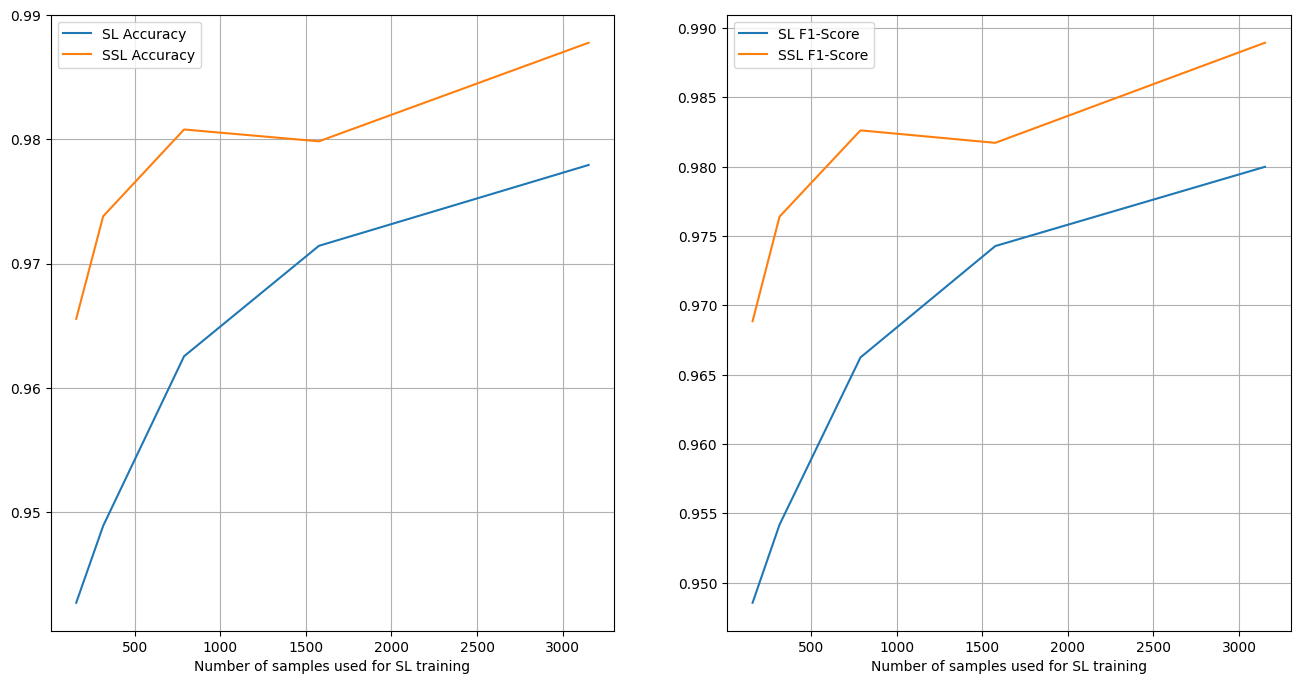
\includegraphics[width=15cm]{img/resnet.png}
    \caption{ResNet based classifier classification performance based on training samples.}
    \label{resnet_m}
\end{figure}

\begin{figure}[]
    \centering
    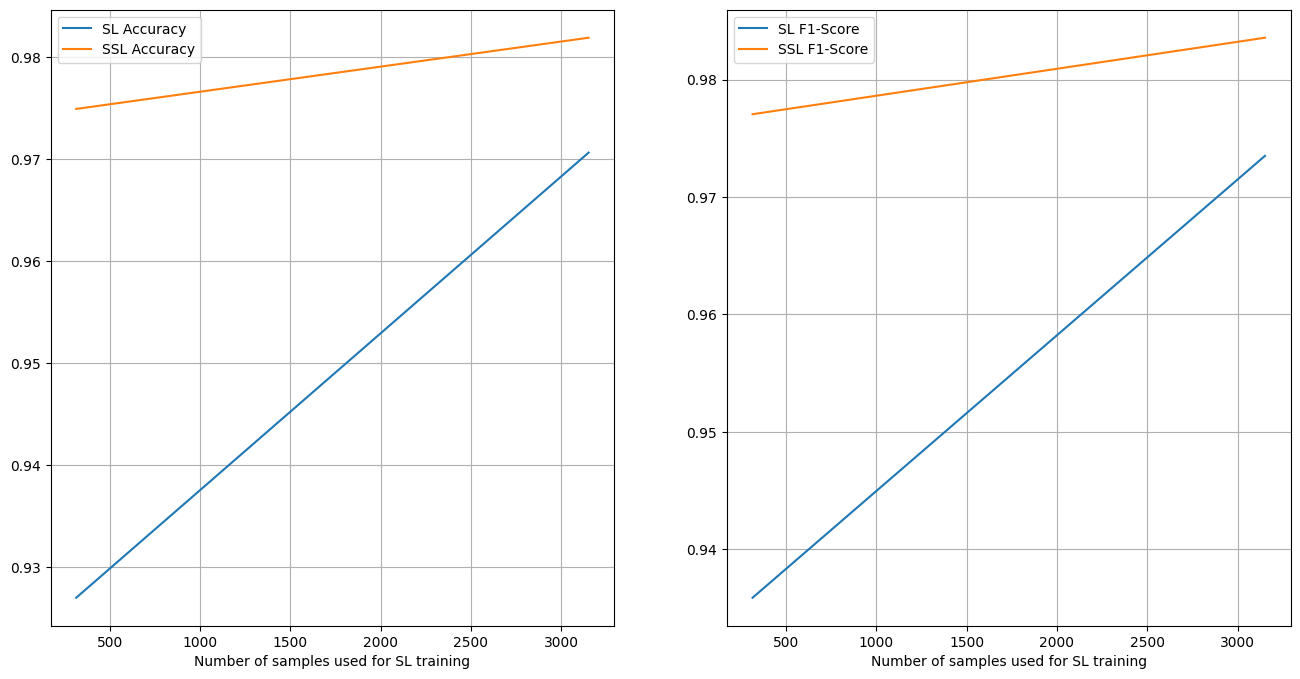
\includegraphics[width=15cm]{img/unet.png}
    \caption{UNet based classifier classification performance based on training samples.}
    \label{unet_m}
\end{figure}

\begin{figure}[]
    \centering
    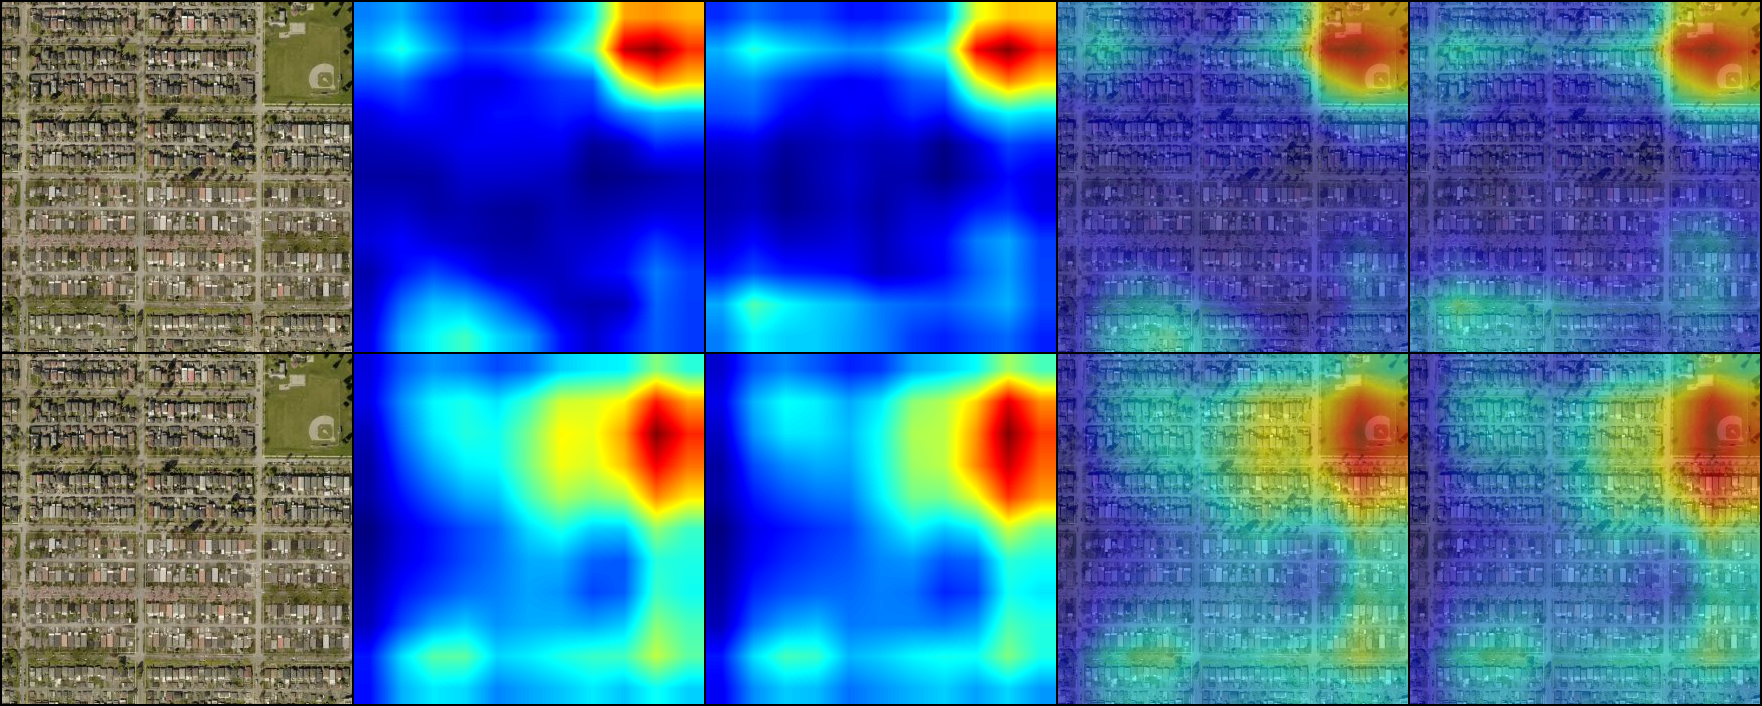
\includegraphics[width=15cm]{img/gradcam_nwf.png}
    \caption{Visual explanation of classification on ResNet based classifier using GradCAM.}
    \label{resnet_g}
\end{figure}

\begin{figure}[]
    \centering
    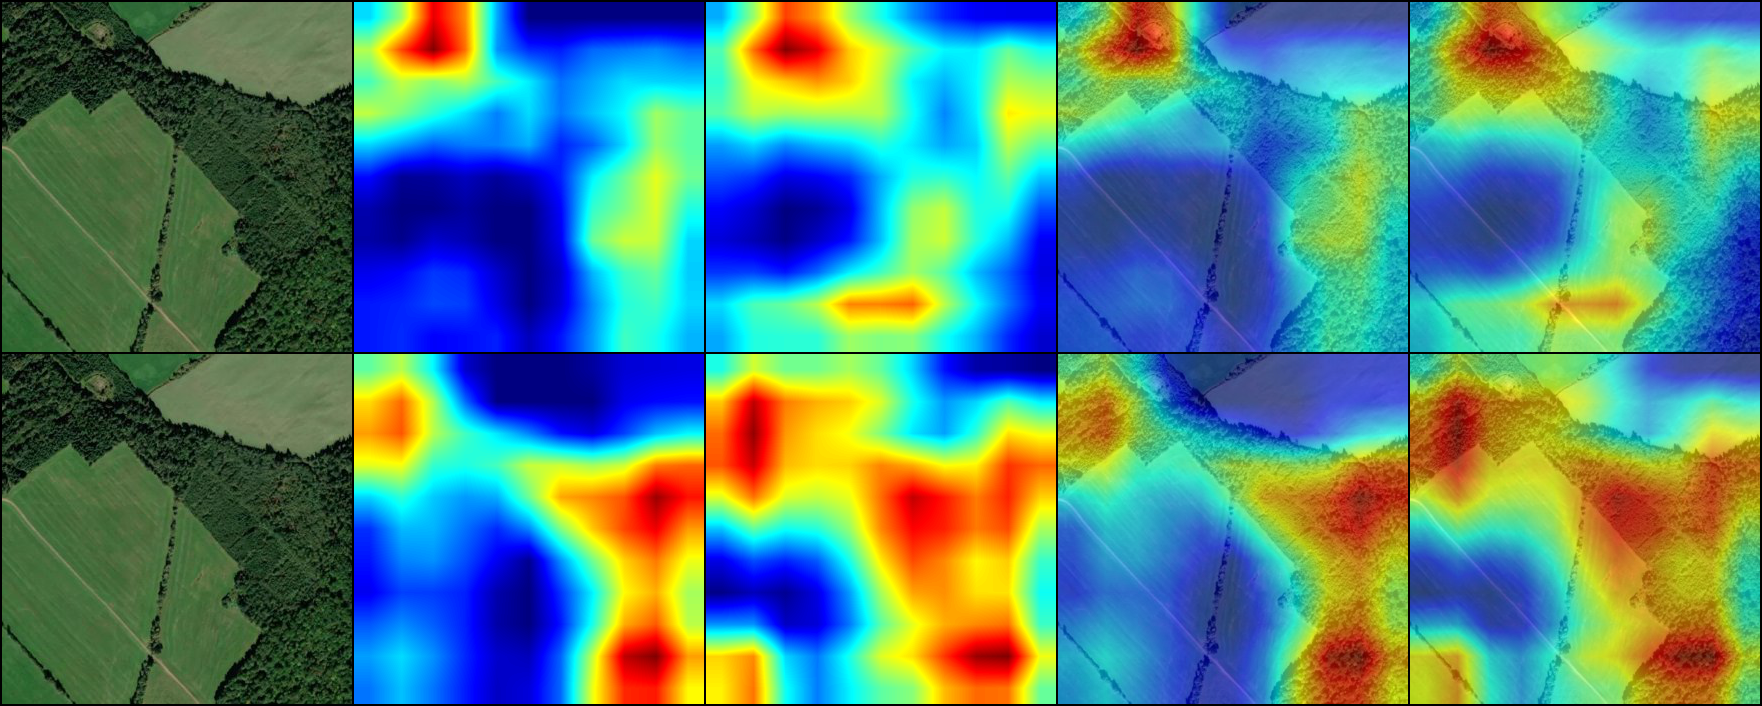
\includegraphics[width=15cm]{img/gradcam_wf.png}
    \caption{Visual explanation of classification on UNet based classifier using GradCAM.}
    \label{unet_g}
\end{figure}

% \begin{figure}[H]
%     \centering
%     \subfloat[\centering \(C1 = 100\), \(C2 = 50\) et \(\lambda = 40\)]{{\includegraphics[scale=0.5]{img.jpg} \label{fig_2:a}}}
%     \qquad
%     \subfloat[\centering \(C1 = 50\), \(C2 = 300\) et \(\lambda = 40\)]{{\includegraphics[scale=0.5]{img.jpg} \label{fig_2:b}}}
%     \caption{Ipsum}
%     \label{fig_2}
% \end{figure}

% \noindent
% \begin{minipage}[!hc]{0.12\textwidth}
%     \begin{flushleft}
%         \textbf{Remarque:}
%     \end{flushleft}
% \end{minipage}
% \vrule\enskip\vrule\quad\begin{minipage}{\dimexpr 0.87\textwidth-0.8pt-1.5em}
%     Lorem ipsum
% \end{minipage}

\end{questions}

\end{document}